\documentclass[authoryear]{elsarticle}

\usepackage{amsmath}
\usepackage{bm}
\usepackage{pgfplots}
\usepackage{color, colortbl}
\usepackage{graphicx}

\graphicspath{{figs/}}

\usepackage{hyperref}
\usepackage{multirow}
\usepackage{float} 

\bibliographystyle{elsarticle-harv}

\begin{document}

\begin{frontmatter}
\title{A generalized multiscale finite element method for neutron transport problems in SP$_3$ approximation}

\author[nefu]{Aleksandr O. Vasilev\corref{cor}}
\ead{haska87@gmail.com}

\author[nefu]{Denis A. Spiridonov}
\ead{d.stalnov@mail.ru}

\author[ki]{Alexander V. Avvakumov}
\ead{Avvakumov2009@rambler.ru}

\address[nefu]{North-Eastern Federal University, 58, Belinskogo, Yakutsk, Russia}
\address[ki]{National Research Center \emph{Kurchatov Institute},  1, Sq. Academician Kurchatov, Moscow, Russia}

\cortext[cor]{Corresponding author}

\begin{abstract}
The SP$_3$ approximation of the neutron transport equation allows improving the accuracy for both static and transient simulations for reactor core analysis compared with the neutron diffusion theory. 
Besides, the SP$_3$ calculation costs are much less than higher order transport methods (S$_N$ or P$_N$).
Another advantage of the SP$_3$ approximation is a similar structure of equations that is used in the diffusion method. 
Therefore, there is no difficulty to implement the SP$_3$ solution option to the multi-group neutron diffusion codes. 

In this paper, we attempt to employ a model reduction technique based on the multiscale method for neutron transport equation in SP$_3$ approximation. 
The proposed method is based on the use of a generalized multiscale finite element method (GMsFEM).
The main idea is to create multiscale basis functions that can be used to effectively solve on a coarse grid.
From calculation results, we obtain that multiscale basis functions can properly take into account the small-scale characteristics of the medium and provide accurate solutions. 
The application of the SP$_3$ methodology based on solution of the $\lambda$-spectral problems has been tested for the some reactor benchmarks.
The results calculated with the GMsFEM are compared with the reference transport calculation results.
\end{abstract}

\begin{keyword}
neutron transport equation, SP3 approximation, eigenvalues, multiscale simulation, generalized multiscale finite element method, GMsFEM
\end{keyword}

\end{frontmatter}

\section{Introduction}
%Among the basic physical processes occurring in a nuclear reactor \cite{Duderstadt1976}, the focus is on neutron transport. 
%To predict the neutron distribution, a rather complex integro-differential equation is involved; besides, the neutron flux distribution depends on time, energy, spatial and angular variables \cite{Stacey2007}.
%In practical calculations of nuclear reactors, as a rule,  different approximative forms of the neutron transport equation are used. For example, the most neutronics codes are based on the multigroup diffusion equations.
%The computational model is a system of coupled second-order parabolic equations, which is supplemented by a system of ordinary differential equations to take into account delayed neutrons.
%
%The stationary state of neutron flux, which is related to the critical state of the reactor, is characterised by local balancing of neutron absorption and generation. 
%This boundary state is usually described by solution of a spectral problem (Lambda Modes problem \cite{Verdu1994, Annals2017, Munoz2019}) provided that the fundamental eigenvalue (maximal eigenvalue) that is called k-effective of the reactor core, is equal to unity. 
%In this case, the stationary neutron field is related with the corresponding eigenfunction.
%Computations of k-effective of the reactor using the Lambda Modes problem are obligatory for reactor design calculations.
%
%Real dynamic neutronic calculations require the use of large computational grids during large characteristic times. For these reasons, the reactor calculations can be very expensive.
%When solving these problems, it is common to use numerical averaging techniques or different multiscale methods that can significantly reduce the number of unknowns, through the construction of coarse-scale model.
%Also note a class of methods for modelling the non-stationary  neutron diffusion, which is associated with the multiplicative representation of the space-time factorization methods and the quasistatic method \cite{dulla2008quasi, Carreno2019}. 
%The general strategy for the approximate solution of the non-stationary problems of neutron transport, which is oriented to fast calculations using the state change modal method was formulated in \cite{Progress2018}.
%
%Homogenization methods are used for coarse-grid approximation and allow calculating the effective properties of the domain.
%As a result, the methods of numerical homogenization establish macroscopic laws on the basis of local computations, but such approaches are usually based on a priori formulated assumptions, see e.g. \cite{Stalnov2017,Bakhvalov2012, Vidal2018}. 
%On the other hand, multiscale methods construct multiscale basis functions in each coarse-grid block and couple these basis functions in a global formulation. 
%These methods have a two-way information exchange between micro- and macro-scales. 
%There are many variations of multiscale finite element methods (MsFEM).
%A detailed description of several variations of the method is presented in \cite{Efendiev2009}.
%
%In this paper, we propose a Generalized Multiscale Finite Element Method (GMsFEM \cite{Efendiev2013, Spiridonov2019}) to solve the neutron diffusion equation. 
%The main idea of the GMsFEM is the dimensionality reduction of the problem. 
%GMsFEM  involves two basic steps: the construction of multiscale basis functions that take into account small scale heterogeneities in local domains and the construction of the coarse scale approximation. 
%For the construction of the multiscale basis functions we solve spectral problems in local domains.
%Spectral problems allow identifying the most important characteristics of the solution. 
%In contrast to the available techniques, this method allows to avoid the limitations associated with idealization and the applicability of the method.
%This method also more general technology that takes into account the different scale processes.
%The construction of basis functions occurs independently for each local domain and doesn't require information exchanges between processors, and the method is effective in a high parallelization.
%Using constructed multiscale basis functions, we construct a mathematical model on a coarse grid that allows to significant reduce the solution time, the amount of used memory, and can be used to perform calculations for a given configuration of  heterogeneous properties. 
%
%In this paper, we present numerical results for 2D small PWR test.
%We compare the GMsFEM results with the fine-grid simulations. 
%In these calculations, we use various number of multiscale basis functions in each local subdomain. 
%As can be seen, as the number of basis functions increases, the multiscale solution becomes more accurate.
%In particular, when we use few functions, the result is not accurate, therefore it necessary to select more basis functions. 
%The errors of the method are shown in $L_2$ and $H_1$ norms. 

%%%%%%%%%%%%%%%%%%%%%%%%%%%%%%%%%%%%%%%%%%%%%%%%%%%%%%%%%%%%%%%%%%

\section{Problem statement}
Let us consider the symmetric form of the SP$_3$ equation for the neutron flux.
The neutron dynamics is considered in the limited convex two-dimensional or three-dimensional area $\Omega$ ($\bm x = \{x_1, ..., x_d\} \in \Omega, \, d = 2,3$) with boundary $\partial \Omega$.
The neutron transport is described by the system of equations
\begin{equation}\label{1}
\begin{split}
	\frac{1}{v_g} \frac{\partial \phi_{0,g}}{\partial t} - 
	\frac{2}{v_g} \frac{\partial \phi_{2,g}}{\partial t} - 
	& \nabla \cdot D_{0,g} \nabla \phi_{0,g} + 
	  \Sigma_{r,g} \phi_{0,g} -  
	2 \Sigma_{r,g} \phi_{2,g} \\ 
	= & (1 - \beta) \chi_{n,g} S_{n} + S_{s,g} + \chi_{d,g} S_d, \\
	- \frac{2}{v_g} \frac{\partial \phi_{0,g}}{\partial t} + 
	  \frac{9}{v_g} \frac{\partial \phi_{2,g}}{\partial t} - 
	& \nabla \cdot D_{2,g} \nabla \phi_{2,g} + 
	5 \Sigma_{t,g} + 4\Sigma_{r,g}) \phi_{2,g} - 
	2 \Sigma_{r,g} \phi_{0,g} \\
	= & - 2(1 - \beta) \chi_{n,g} S_{n} - 2 S_{s,g} - 2 \chi_{d,g} S_d,
\end{split}
\end{equation}
where
\[
	S_{n} = \sum_{g'=1}^{G} \nu \Sigma_{f,g'} \phi_{g'}, \quad
	S_{s,g} = \sum_{g\neq g'=1}^{G} \Sigma_{s,g' \rightarrow g} \phi_{g'}, \quad
	S_{d} = \sum_{m=1}^{M} \lambda_m c_m,
\]
\[
	\phi_{0,g} = \phi_g + 2\phi_{2,g}, \quad
	D_{0,g} = \cfrac{1}{3 \Sigma_{tr,g}}, \quad
	D_{2,g} = \cfrac{9}{7 \Sigma_{t,g}}, \quad 
	g = 1,2,\dots,G.
\]
Here $G$ --- number of energy groups,
$\phi_g(\bm x, t)$ --- scalar flux,
$\phi_{0,g}(\bm x, t)$ --- pseudo 0th moment of angular flux,
$\phi_{2,g}(\bm x, t)$ --- second moment of angular flux,
$\Sigma_{t,g}(\bm x, t)$ --- total cross-section,
$\Sigma_{tr,g}(\bm x, t)$ --- transport cross-section, 
$\Sigma_{r,g}(\bm x, t)$ --- removal cross-section,
$\Sigma_{s,g' \rightarrow g}(\bm x, t)$ --- scattering cross-section,
$\chi_g$  --- spectra of neutrons,
$\nu \Sigma_{f,g}(\bm x, t)$ --- generation cross-section,
$c_m(\bm x, t)$ --- density of sources of delayed neutrons,
$\lambda_m$ --- decay constant of sources of delayed neutrons,
$M$ --- number of types of delayed neutrons.

The density of sources of delayed neutrons is described by the equations
\begin{equation}\label{2}
	\frac{\partial c_m}{\partial t} + \lambda_m c_m = \beta_m S_{n}, \quad m = 1,2,\dots,M,
\end{equation}
where $\beta_m$ is the fraction of delayed neutrons of m-type, and
\[
	\beta = \sum_{m=1}^{M} \beta_m.
\] 
The Marshak-type conditions are set at the boundary of the area $\partial \Omega$
\begin{equation}\label{3}
\begin{split}
	\begin{bmatrix}
		J_{0,g}(\bm x) \\
		J_{2,g}(\bm x) \\
	\end{bmatrix}
	=
	\begin{bmatrix}
		\phantom{-} \cfrac{1}{2} & - \cfrac{3}{8} \\
	    -\cfrac{3}{8} & \phantom{-} \cfrac{21}{8} \\
	\end{bmatrix}
	\begin{bmatrix}
		\phi_{0,g}(\bm x) \\
		\phi_{2,g}(\bm x) \\
	\end{bmatrix}, \\
	J_{i,g}(\bm x) = - D_{i,g} \nabla \phi_{i,g}(\bm x), \quad i = 0, 2.
\end{split}
\end{equation}

System of equations \eqref{1} and \eqref{2} is supplemented with boundary conditions \eqref{3} and corresponding initial conditions
\begin{equation}\label{4}
\begin{split}
	\phi_g(\bm x,0) & = \phi_g^0(\bm x), \quad g = 1,2,\dots,G, \\ 
	\quad c_m(\bm x,0) & = c_m^0(\bm x), \quad m = 1,2,\dots,M.
\end{split}
\end{equation}
We assume that at the initial time t = 0, the reactor is in steady-state critical condition.

\textbf{Discretization.}
Let's discretize the boundary problem \eqref{1}-\eqref{4}.
Define a uniform grid
\[
	\omega = \{ t^n=n \tau, \quad n = 0,1,\dots,N, \quad \tau N = T \}
\]
and use the next notations $\phi^n_g = \phi_g(\bm{x}, t^n)$, $c^n_m = c_m(\bm{x}, t^n)$. 
We discretize the time derivatives of equation \eqref{1} using finite-difference scheme. 
For approximation in time, we use a fully implicit scheme with time step $\tau$.
For delayed neutron source equation we use numerical-analytical method for the construction of approximations in time.
The equation \eqref{2} in the equivalent form
\[
	\frac{\partial e^{\lambda_m t} c_m}{\partial t} = 
	\beta_m e^{\lambda_m t} \sum_{g=1}^{G} \nu \Sigma_{fg} \phi_g, \quad m = 1,2,\dots,M.
\]
After integration on time interval $[t^n, t^{n+1}]$ one can obtained
\begin{equation}\label{5}
	c_m^{n+1} = e^{-\lambda_m\tau} c_m^n + 
	\beta_m \int_{t_n}^{t_{n+1}} e^{\lambda_m (t - t^{n+1})} \sum_{g=1}^{G} \nu \Sigma_{fg} \phi_g d t,
	\quad m = 1,2,\dots,M.
\end{equation}
When using the fully implicit scheme, we take the integrand on the right-hand side of \eqref{5} at $t = t^{n + 1}$.

For spatial approximation we use the finite element method.
Let $H^1(\Omega)$ -- Sobolev space, $q \in H^1$: $q^2$ and $\vert\nabla q\vert^2$ have a finite integral in $\Omega$. 
Using the integration by parts, we obtain the following variational formulation: let's find $\phi^{n+1}_g \in V^G$ such that
\begin{equation}\label{6}
\begin{split}
	\int_{\Omega} 
		\left( 
			\frac{\phi^{n+1}_{0,g} - \phi^{n}_{0,g}}{v_g \tau} -
			\frac{2(\phi^{n+1}_{2,g} - \phi^{n}_{2,g})}{v_g \tau} 
		\right) q_g d\bm{x} - & %centering
	\int_{\Omega} D_{0,g} \nabla \phi^{n+1}_{0,g} \nabla q_g d\bm{x} \\
	+ \int_{\partial\Omega} J^{n+1}_{0,g} q_g d\bm{s} +
	\int_{\Omega}
		(
			\Sigma_{r,g} \phi^{n+1}_{0,g} - & %centering
			2\Sigma_{r,g} \phi^{n+1}_{2,g} 
		) q_g d\bm{x} \\
	= \int_{\Omega} 
		(
			(1 - \beta) \chi_{n,g} S^{n+1}_{n} + 
			 S^{n+1}_{s,g} + & %centering
			 \chi_{d,g} S^{n+1}_d 
		) q_g d\bm{x}, \\
	\int_{\Omega} 
		\left( 
			- \frac{2(\phi^{n+1}_{0,g} - \phi^{n}_{0,g})}{v_g \tau} + 
			\frac{9(\phi^{n+1}_{2,g} - \phi^{n}_{2,g})}{v_g \tau} 
		\right) q_g d\bm{x} - & %centering
	\int_{\Omega} D_{2,g} \nabla \phi^{n+1}_{2,g} \nabla  q_g d\bm{x} \\
	+ \int_{\partial\Omega} J^{n+1}_{2,g} q_g d\bm{s} + 
	\int_{\Omega} 
		( 
			(5 \Sigma_{t,g} + 
			4 \Sigma_{r,g}) \phi^{n+1}_{2,g} - & %centering
			2\Sigma_{r,g} \phi^{n+1}_{0,g} 
		) q_g d\bm{x} \\
	= \int_{\Omega}
		( 
			- 2(1 - \beta) \chi_{n,g} S^{n+1}_{n} - 
			2S^{n+1}_{s,g} - & %centering
			2\chi_{d,g} S^{n+1}_d 
		) q_g d\bm{x},
\end{split}
\end{equation}
where $V^G=[H^1(\Omega)]^G$.

Further, it's necessary to pass from the continuous variational problem \eqref{6} to the discrete problem. 
We introduce finite-dimensional space of finite elements $V^G_h \subset V^G$ and formulate a discrete variational problem. 
We use standard linear basis functions as basis functions to solve the problem on the fine grid.
The problem is solving a system of linear algebraic equations
\begin{equation}\label{7}
	A_f \phi = b_f,
\end{equation}
where the operator $A_f$ corresponds to the bilinear form of equation, and the vector $b_f$ corresponds to the linear form of equation \eqref{6}.

\section{Multiscale method}
For the discretization on the coarse grid we use GMsFEM.
We construct two grids: fine grid ($\mathcal{T}_h$) and coarse grid ($\mathcal{T}_H$) (see Figure \ref{p1}).
For multiscale basis construction, we define local domains $\omega_i$, where $i = 1,..., N_v$ and $N_v$ is the number of coarse grid nodes.
We assume that $\mathcal{T}_h$ is a refinement of $\mathcal{T}_H$, where $h$ and $H$ represent the fine and coarse grid sizes, respectively. 
We assume that the fine-scale grid $\mathcal{T}_h$ is sufficiently fine to fully resolve the small-scale information of the domain  while $\mathcal{T}_H$ is a coarse grid containing many fine-scale features.
A local domain $\omega_i$ is obtained by the combining all the coarse cells around one vertex of the coarse grid. 

\begin{figure}[ht]
	\centering
		
\includegraphics[width=0.3\linewidth]{coarse_grid.png} \hspace{2em}
		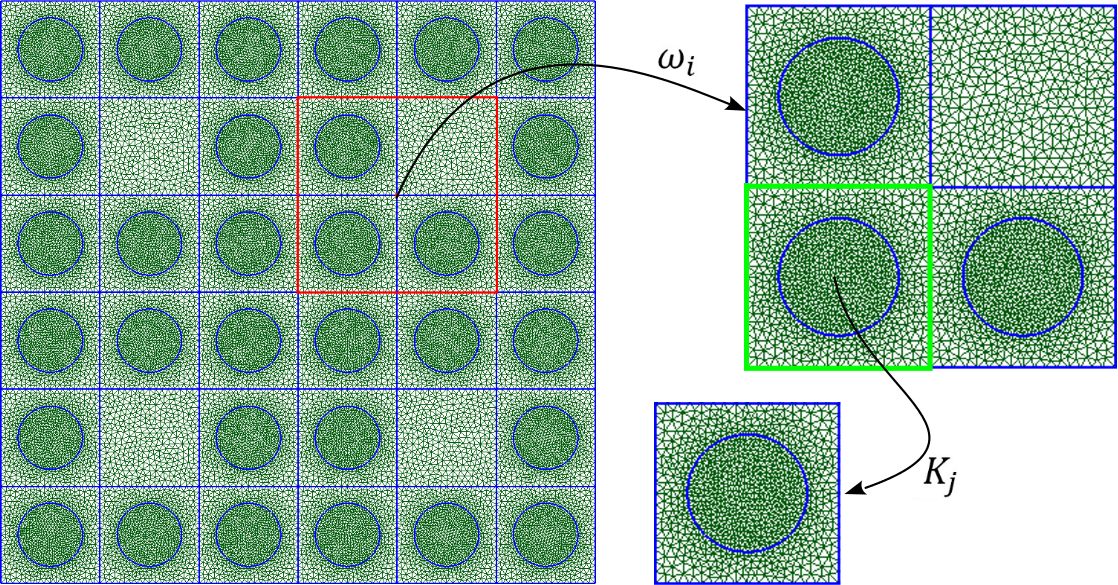
\includegraphics[width=0.57\linewidth]{omega.png} 
	\caption{Coarse grid and local domain $\omega_i$ with $K_j$}
	\label{p1}
\end{figure} 

We construct the multiscale function spaces
\[
	{V}_{\text{off}} = \mbox{span} \{y_{j}\}_{j=1}^{N},
\]
where $N$ is the number of coarse basis functions.
Each $y_j$ is supported in local domain $w_i$.

Basis functions are designed to capture the multiscale features of the solution. 
Important multiscale features of the solution are incorporated into localized basis functions which contain information about the scales that are smaller (as well as larger) than the local numerical scale defined by the basis functions. 
 
% spectral
\textbf{Multiscale space.}
The computation of basis functions use local spectral problems to reduce the dimension of the local problem. 
In order to construct conforming basis functions, we multiply eigenvectors related to dominant eigenvalues to the partition of unity functions.
We use following spectral problem in $\omega_i$
\begin{equation}\label{8}
	A \varphi^i = \lambda S \varphi^i,
\end{equation} 
where the elements of the matrices $A = \{a_{ij}\}$ and $S = \{s_{ij}\}$ are defined as follow{
\begin{equation}\label{9}
\begin{split}
	a_{ij} = 
	\int_{\omega_i} \\
	s_{ij} & = \int_{\omega _i}
\end{split}
\end{equation}}
Then, we choose eigenvectors corresponding to dominant $M_{i}$ eigenvalues from \eqref{8} and use them to construct the multiscale basis functions.

% POU
As partition of unity functions, we use linear functions in each domain $\omega_i$.
Partitions of unity are calculated in the domain $K_j$ as a linear function from $\Gamma$ to the vertex $A$, and $0$ is assigned to the entire segment $\Gamma$, and at point $A$ is assigned the value $1$. 
Thus, we obtain a linear function from $0$ to $1$ over the entire domain $K_j$. 
Partitions of unity are shown in Figure \ref{p2}. 
Domain $K_j$ is one element from a coarse grid. 

\begin{figure}[ht]
	\centering
		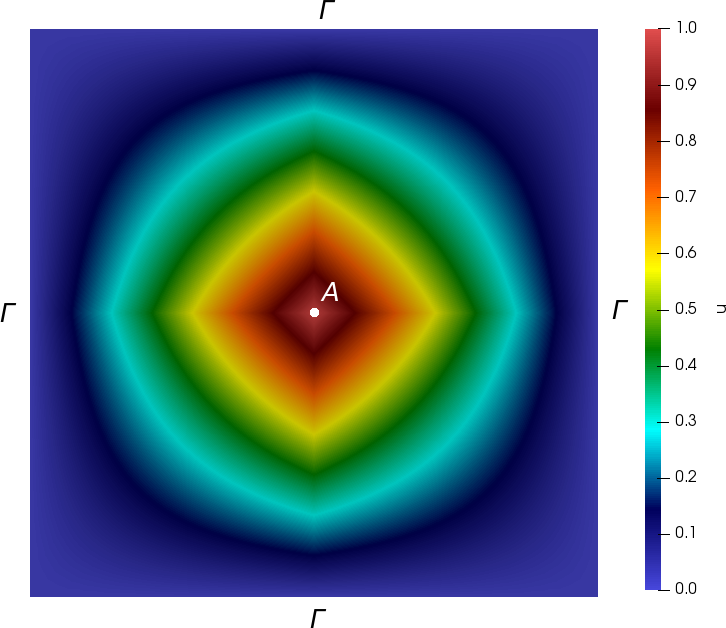
\includegraphics[width=0.45\linewidth]{pofs.png} \hspace{2em}
		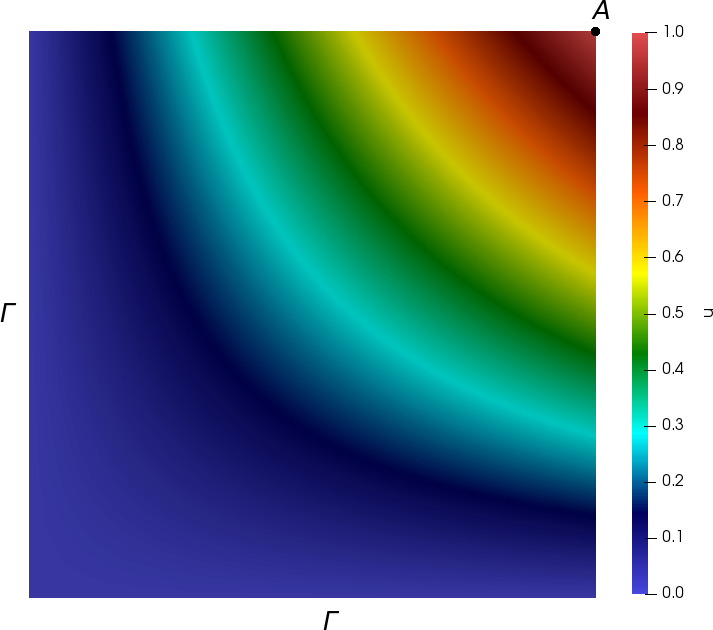
\includegraphics[width=0.45\linewidth]{pouK.png} 
	\caption{Partition of unity functions on the $\omega_i$ (right) and $K_j$ (left)}
	\label{p2}
\end{figure} 
 
The multiscale space is defined as the span of $y_i = \chi_i \varphi^i_k$, where $\chi_i$ is the usual nodal basis function for the node $i$ (linear partition of unity functions). 
The number of bases can be different, the accuracy of the solution can be improved when we increase the number of bases.

% Assembling a matrix in a multiscale space
\textbf{Coarse-scale approximation.}
Next, we create the following matrix for each $\omega_i$
\[
	R^i = \left[ y_1, \dots, y_{M_i-1},  y_{M_i} \right].
\]
and define the transition matrix from a fine grid to a coarse grid $R$ to reduce the dimension of the problem
\[
	R = [R^1, R^2, \dots, R^{N_v}],
\]
where $N_v$ is the number of local domains $\omega_i$.

Then using the transition matrix $R$ and fine grid system \eqref{7}, we construct the coarse grid approximation
\[
	A_c \phi_c = b_c, \quad 
	A_c = R A_f R^T \quad 
	\text{and} \quad 
	b_c = R b_f,
\]
and using the coarse-scale solution $\phi_c$, we can reconstruct the fine grid solution 
\[
	\phi_{ms} = R^T \phi_c.
\]

\section{Numerical results}
%Проводится численное моделирование нестационарных тестов в транспортном SP_$3$ приближении.
%Исследуются и сравниваются численные результаты полученные методом конечных элементов и обобщенным многомасштабным методом конечных элементов.
%Программное обеспечение написано с использованием вычислительной платформы FEniCS. 
%Для решения спектральных задач с несимметричными матрицами применяется библиотека SLEPc. 
Numerical modeling of non-stationary tests is carried out in the transport SP$_3$ approximation.
Numerical results obtained by the finite element method and the generalized multiscale finite element method are analyzed and compared.
The software has been written using the library FEniCS.
SLEPc library has been used to solve spectral problems with asymmetric matrices.

At each time the integrated power is calculated as
	\[P(t) = a \int_{\Omega} \sum_{g=1}^{G} \Sigma_{f,g} \phi_g d \bm x,\]
where $a$ is the normalization coefficient, which corresponds to a given value of the integrated power.

\subsection{One group heterogeneous test}
Let's consider the 2D test problem for small PWR reactor ($\Omega$ --- reactor core area). 
The geometrical model of the small PWR reactor core is presented in Fig.\ref{p3}. 
The diameter of the fuel rods is 0.82 cm, the cell width is 1.26 cm.
Neutronics constants in the common notations are given in Table \ref{t1}. 
There are two types of cassettes, with fuel 1\% $UO_2$ and 2\% $UO_2$.
The following delayed neutrons parameters are used: $\beta = 6.5 \cdot 10^{-3}$, $\lambda = 0.08$ s$^{-1}$ and $v = 5 \cdot 10^5$ cm/s.

\begin{figure}[ht]
	\centering
	    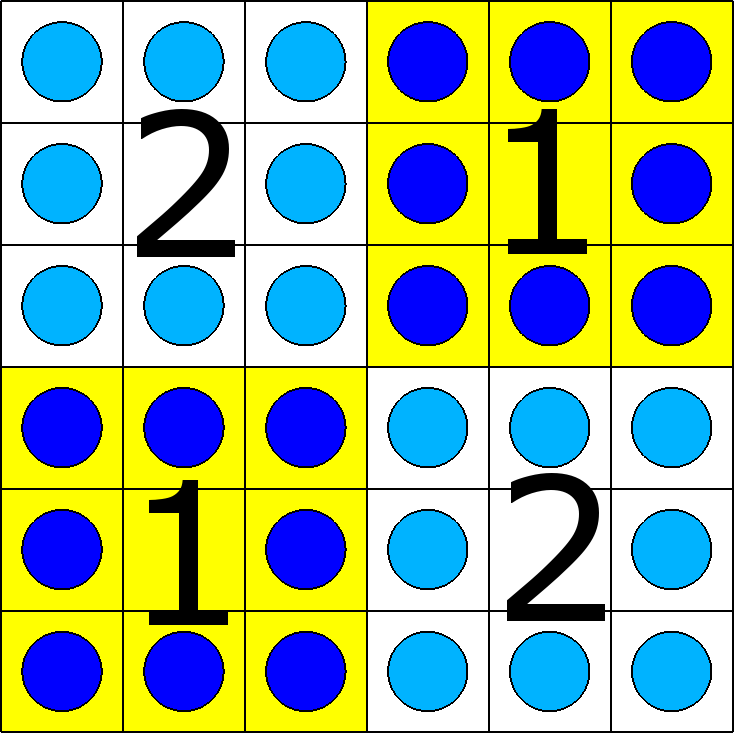
\includegraphics[width=0.5\linewidth] {smallpwr.png}
	\caption{Geometrical model of the small PWR-2D reactor core}
	\label{p3}
\end{figure} 

We define the next scenario of the process:
\begin{itemize}
\item The $\lambda$-spectral problem is solved and the solution is taken as the initial condition;
\item Calculation for the non-stationary model at the time range from 0 to 0.4 sec;
\item At $t=0.1$ sec and $t=0.3$ sec $\Sigma_a$ for fuel in the zone 1 changes to +2\% and -3\%, respectively (simulation of insertion or withdrawal of control rods).
\end{itemize}

\begin{table}[ht]
\caption{Neutronics constants for small PWR-2D.}
\label{t1}
\begin{center}
\begin{tabular}{l l l l l l}
\hline
\multirow{2}{*}{} & \multicolumn{2}{c}{1} & \multicolumn{2}{c}{2} \\
\cline{2-5}
& coolant & fuel & coolant & fuel \\
\hline
	$D$          & 3.4473872E-01 & 7.7002585E-01 & 3.1679441E-01 & 8.0236505E-01    \\
	$\Sigma_t$   & 9.6691584E-01 & 4.3288590E-01 & 1.0522071E+00 & 4.1543850E-01    \\
	$\Sigma_r$   & 5.3858400E-03 & 8.9337900E-02 & 6.0670900E-03 & 6.6279500E-02 \\
	$\Sigma_{f}$ & 0.0           & 5.4731800E-02 & 0.0           & 3.3377700E-02 \\
	$\nu$        & 0.0           & 2.44844862    & 0.0           & 2.45482762    \\
\hline
\end{tabular}
\end{center}
\end{table}

The coarse grid contains $49$ vertices.
The fine grid contains 115891 vertices. 
The time step for both grids is $\tau = 0.001$.
As an exact solution, we take the fine-grid solution.
The initial value of $K_{eff}$ is 1.xxxxxx. 

\begin{figure}[ht]
	\centering
		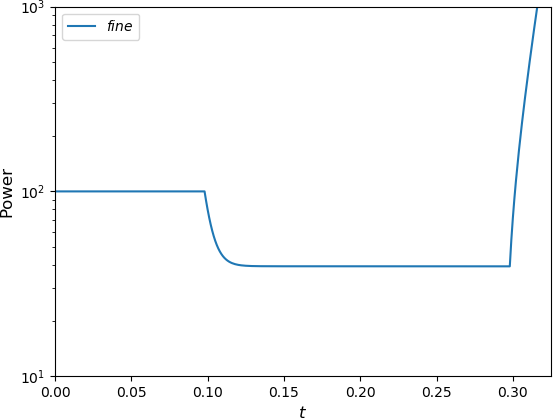
\includegraphics[width=0.45\linewidth]{power_fine.png} \hspace{2em}
		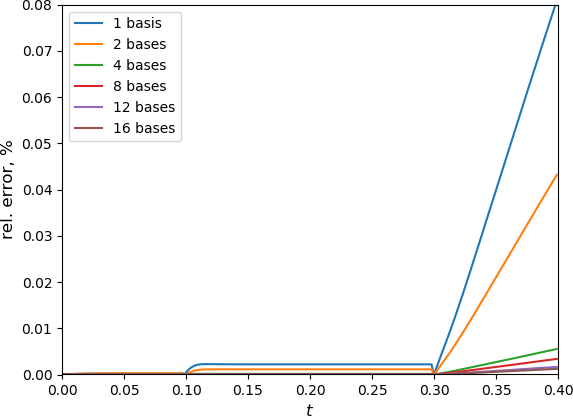
\includegraphics[width=0.45\linewidth]{power.png}
	\caption{Integral power (fine grid) and relative errors ($\%$) of the multiscale solution power.}
	\label{p4}
\end{figure}
 
The integral power for the fine grid and relative errors of integral powers are shown in Figure~\ref{p4}.
When using single basis, the error does not exceed 1\%, and for using 4 or more bases it does not exceed 0.01\%.

In Figure~\ref{p5}, we present relative $L_2$ and $H_1$ errors of the multiscale solution vs. time for different number of multiscale basis functions.
The numerical results show good convergence behaviour, provided that we take sufficient number of the multiscale basis functions.

\begin{figure}[ht]
	\centering
		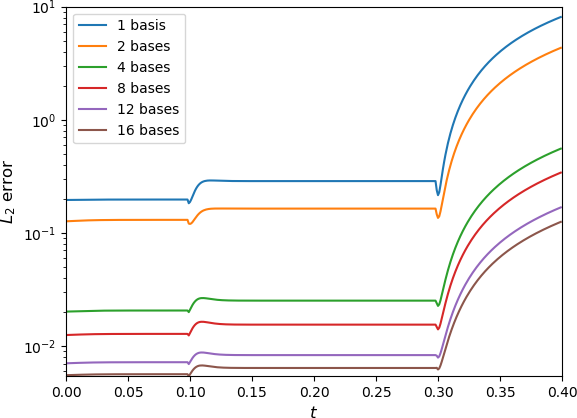
\includegraphics[width=0.45\linewidth]{L2_log.png} \hspace{2em}
		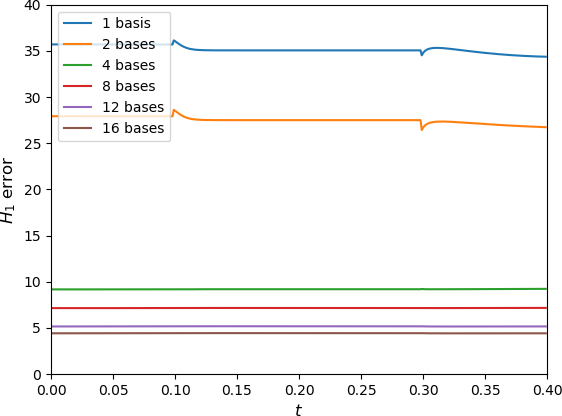
\includegraphics[width=0.45\linewidth]{H1.png}
	\caption{Relative $L_2$ and $H_1$ errors ($\%$) of the multiscale solution.}
	\label{p5}
\end{figure}

In Table~\ref{t2}, we present relative $L_2$ and $H_1$ errors at final time for different number of the multiscale basis functions.
For example, when we use 8 spectral basis functions, we obtain $0.34\%$ for $L_2$ error and $7.18\%$ for $H_1$ error.
Our calculations show that it is necessary to use 4 or more basis functions.
In Figure~\ref{p7}, we present first four (of 16) multiscale basis functions in local domain $\omega_i$.
The fine-grid solution and the multiscale solution (16 basis functions on each local domain) $\omega_i$ are shown in Figure \ref{p6}. Relative errors are 0.13\% for $L_2$ and 4.43\% for $H_1$.

\begin{table}[ht]
	\caption{Relative $L_2$ and $H_1$ errors ($\%$) of the solution at final time.}
	\label{t2}
	\begin{center}
		\begin{tabular}{ c c r r r }
			\hline
			Number of bases & Number of DOF & $L_2$ error & $H_1$ error & Calc time\\
			\hline
			1 & 49 & 8.09 & 34.36 & 0.015 \\
			2 & 98 & 4.32 & 26.73 & 0.018 \\
			4 & 196 & 0.56 & 9.24 & 0.026 \\
			8 & 392 & 0.34 & 7.18 & 0.056 \\
			12 & 588 & 0.17 & 5.17 & 0.102 \\
			16 & 784 & 0.13 & 4.43 & 0.239 \\
			fine & 115891 & -- & -- & 6.816 \\
			\hline
		\end{tabular}
	\end{center}
\end{table}

\begin{figure}[h!]
	\centering
		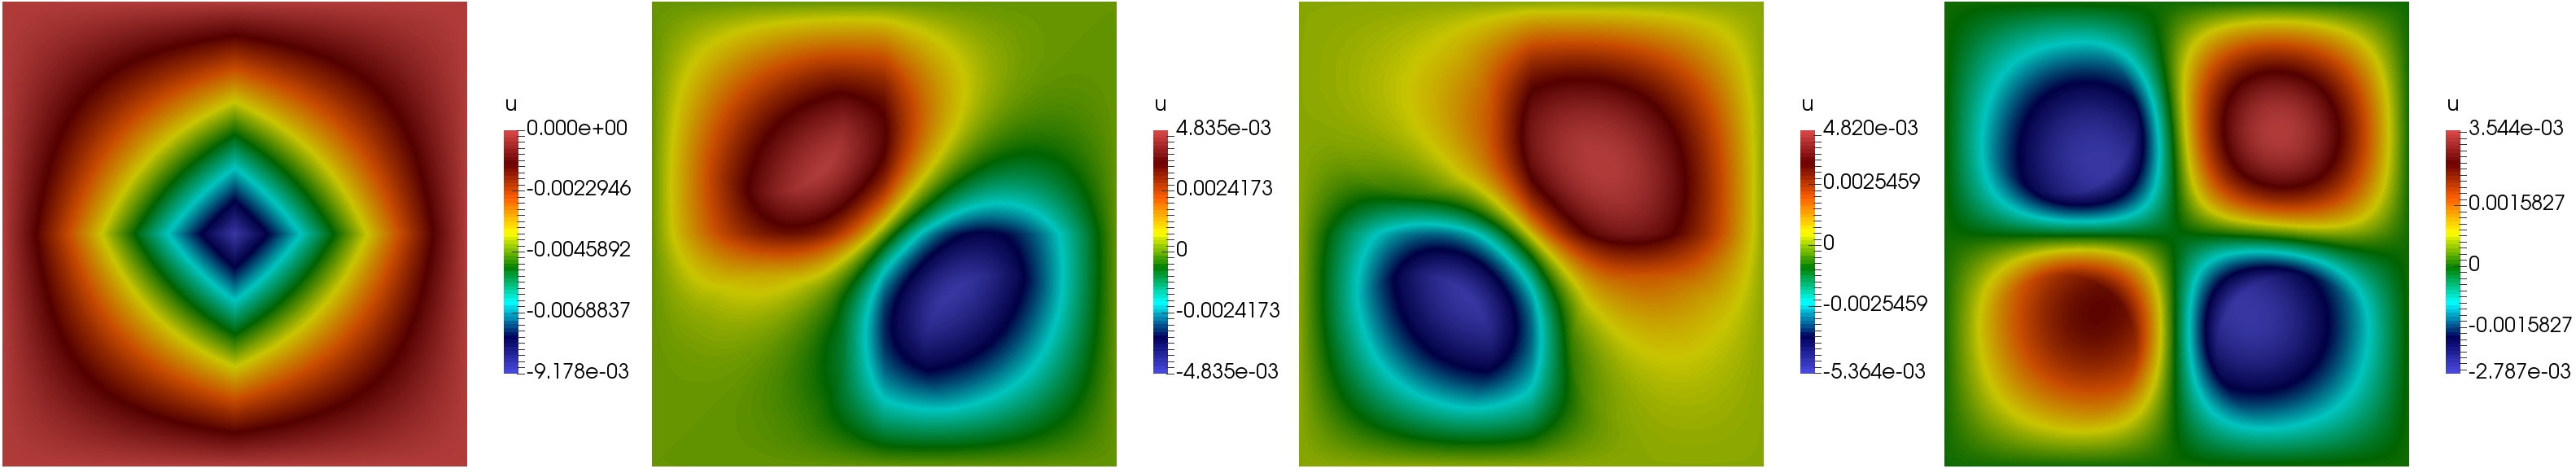
\includegraphics[width=0.95\linewidth]{basis.png}
	\caption{The first four multiscale basis functions.}
	\label{p7}
\end{figure}

\begin{figure}[h!]
	\centering
		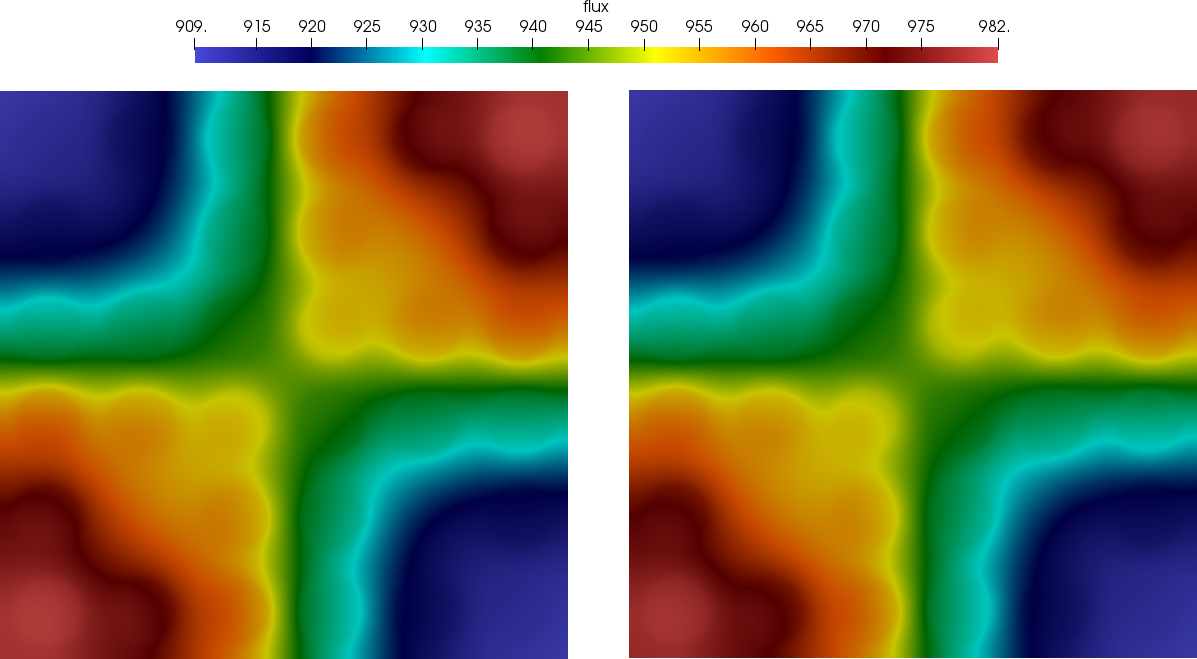
\includegraphics[width=0.75\linewidth]{flux.png}
	\caption{Fine grid and multiscale solution with 16 basis functions at final time.}
	\label{p6}
\end{figure}

\subsection{two group test}
%Рассматривается двумерный транспортный тест \cite{hageman1969}. 
%Моделируется 1/4 часть активной зоны реактора, размеры которой составляют 160x160 см.
%На рисунке \ref{ris:twigl} показана геометрическая модель активной зоны, где цифрами показаны материалы различных сортов.
%На внешней границе активной зоны реактора задается условие границы с вакуумом.  
%
%Нейтронно-физические константы теста в общепринятых единицах представлены в таблице \ref{table:coeff}. 
%Среднегрупповые скорости нейтронов в тесте одинаковы для всей среды и составляют $v_1 = 10^7$ см/с и $v_2 = 2 \cdot 10^5$ см/с. 
%Спектр деления для мгновенных и запаздывающих нейтронов также одинаков для всей среды и равен $\chi_1 = 1$ и $\chi_2 = 0$.
%В тесте представлена одна эффективная группа запаздывающих нейтронов. 
%Эффективная доля запаздывающих нейтронов составляет $\beta = 0.0075$, а постоянная распада предшественников запаздывающих нейтронов $\lambda = 0.08$ с$^{-1}$. 

\begin{figure}[ht]
\begin{center}
	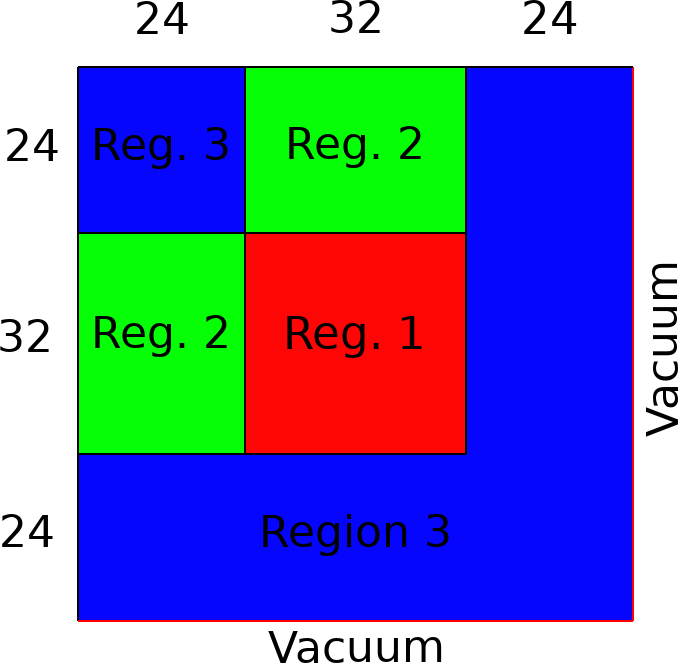
\includegraphics[width=0.5\linewidth]{twigl.png} \\
	\caption{\label{image:canonsummary}Geometrical model of 1/4 reactor core TWIGL-2D.}
	\label{ris:twigl}
\end{center}
\end{figure}

\begin{table}[ht]
\caption{\label{table:coeff}Neutronics constants for TWIGL-2D.}
	\label{t2}
	\begin{center}
	\begin{tabular}{l l l l}
		\hline
		Material & 1 & 2 & 3\\
		\hline 
		$\Sigma_{t,1}$				& 0.2481 & 0.2481 & 0.2644 \\
		$\Sigma_{t,2}$				& 0.9833 & 0.9833 & 0.7167 \\
		$\Sigma_{r,1}$				& 0.01   & 0.01   & 0.008  \\
		$\Sigma_{r,2}$				& 0.15   & 0.15   & 0.05   \\
		$\Sigma_{s,1\rightarrow2}$ 	& 0.01   & 0.01   & 0.01   \\
		$\Sigma_{s,1\rightarrow1}$	& 0.2281 & 0.2281 & 0.2464 \\
		$\Sigma_{s,2\rightarrow2}$	& 0.8333 & 0.8333 & 0.6667 \\
		$\nu_1\Sigma_{f,1}$			& 0.007  & 0.007  & 0.003  \\
		$\nu_2\Sigma_{f,2}$			& 0.2    & 0.2    & 0.06   \\
		\hline
	\end{tabular}
	\end{center}
\end{table}

\section{Conclusions}
A Generalized Multiscale Finite Element method was developed successfully for modelling neutron transport in one-group SP$_3$ approximation.  
We presented an implementation of GMsFEM. 
We considered each step of GMsFEM algorithm.
The results showed that GMsFEM performed with a good accuracy in all considered cases.

In the current work, we considered a popular and simple model of neutron transport equation.
Computational expenses are always an issue even for modern computers.
In the future, we will consider more complex models of neutron transport, such as P$_N$ approximation. 

%\section*{Acknowledgements}
%This work was supported by the grant of the Russian Science Foundation (\#19-71-00008).

% \begin{thebibliography}{16}
%\bibitem{Duderstadt1976}
%Duderstadt J. J. Nuclear reactor analysis. – Wiley, 1976.
%
%\bibitem{Stacey2007}
%Stacey W. M. Nuclear reactor physics. – Weinheim : wiley-vch, 2007. – V. 2.
%
%\bibitem{Annals2017}
%Avvakumov A. V. et al. Spectral properties of dynamic processes in a nuclear reactor //Annals of Nuclear Energy. – 2017. – V. 99. – P. 68-79.
%
%\bibitem{Verdu1994}
%Verdú G. et al. 3D $\lambda$-modes of the neutron-diffusion equation //Annals of Nuclear Energy. – 1994. – V. 21. – №. 7. – P. 405-421.
%
%\bibitem{Munoz2019}
%Munoz-Cobo J. L. et al. 3D calculation of the lambda eigenvalues and eigenmodes of the two-group neutron diffusion equation by coarse-mesh nodal methods //Progress in Nuclear Energy. – 2019. – V. 110. – P. 393-409.
%
%\bibitem{dulla2008quasi}
%Dulla S., Mund E. H., Ravetto P. The quasi-static method revisited //Progress in Nuclear Energy. – 2008. – V. 50. – №. 8. – P. 908-920.
%
%\bibitem{Carreno2019}
%Carreño A. et al. Modal methods for the neutron diffusion equation using different spatial modes //Progress in Nuclear Energy. – 2019. – V. 115. – P. 181-193.
%
%\bibitem{Progress2018}
%Avvakumov A. V. et al. State change modal method for numerical simulation of dynamic processes in a nuclear reactor //Progress in Nuclear Energy. – 2018. – V. 106. – P. 240-261.
%
%\bibitem{Stalnov2017}
%Vasilyeva M., Stalnov D. A. Numerical averaging for the heat conduction problem in inhomogeneous and perforated media //Herald of MK Ammosov Northeastern Federal University. – 2017.
%
%\bibitem{Bakhvalov2012}
%Bakhvalov N. S., Panasenko G. Homogenisation: averaging processes in periodic media: mathematical problems in the mechanics of composite materials. – Springer Science \& Business Media, 2012. – V. 36.
%
%\bibitem{Vidal2018}
%Vidal-Ferràndiz A. et al. Pin-wise homogenization for SPN neutron transport approximation using the finite element method //Journal of Computational and Applied Mathematics. – 2018. – V. 330. – P. 806-821.
%
%\bibitem{Efendiev2009}
%Efendiev Y., Hou T. Y. Multiscale finite element methods: theory and applications. – Springer Science \& Business Media, 2009. – V. 4.
%
%\bibitem{Efendiev2013}
%Efendiev Y., Galvis J., Hou T. Y. Generalized multiscale finite element methods (GMsFEM) //Journal of Computational Physics. – 2013. – V. 251. – P. 116-135.
%
%\bibitem{Spiridonov2019}
%Spiridonov D., Vasilyeva M., Leung W. T. A Generalized Multiscale Finite Element Method (GMsFEM) for perforated domain flows with Robin boundary conditions //Journal of Computational and Applied Mathematics. – 2019. – V. 357. – P. 319-328.
%
%\bibitem{Brenner2007}
%Brenner S., Scott R. The mathematical theory of finite element methods. – Springer Science \& Business Media, 2007. – V. 15.
%
% \bibitem{Forget2005}
% Forget B., Rahnema F. 3-D heterogeneous coarse-mesh transport method. France: N. p., 2005

% \end{thebibliography}

\end{document}
